\documentclass{article}
\usepackage{graphicx} % Required for inserting images
\title{D3: Documento di Architettura}
\author{G06}
\usepackage{fancyhdr}
\usepackage{hyperref}
\newcommand{\myheaderimage}{
\includegraphics[width=2cm]{D3/Images/LogoEasyLib.png}}
\pagestyle{fancy}
\fancyhf{} % Clear the header and footer
\lhead{\myheaderimage} % Place the image in the top right corner
\setlength{\headheight}{3cm} % Adjust the height as needed
\rhead{D3-G06}


\begin{document}

\maketitle

\tableofcontents
\newpage

\section{Scopo del componente}

Il presente documento ha lo scopo di descrivere l’architettura dell’applicazione EasyLib.
Per riuscire a fare ciò, è stato usato un diagramma delle classi utilizzando UML (Unified Modeling Language) e del codice in OCL (Object Constraints Language) per riuscire a chiarire ogni modalità d’uso delle classi all’interno del diagramma. Molte classi sono derivate dai documenti precedenti, in particolare la maggior parte delle classi viene ricavata dal diagramma dei componenti e dal diagramma di contesto; qui ogni classe o gruppo di classe viene analizzato singolarmente o nel suo ambito e poi alla fine viene visualizzato il diagramma completo con anche il codice OCL.

\section{Tipi introdotti}
In questa sezione vengono descritti i tipi introdotti in questo documento che hanno lo scopo di semplificare e aiutare le interazioni tra le classi ricavate dai documenti precedenti.

\begin{enumerate}
    \item \textbf{Data:} Viene introdotto il tipo Data, contenente solo gli attributi giorno, mese anno, di tipo intero. Questa classe è utile all’interno di tutto il diagramma quando viene richiesta una datazione (i.e. data di reso)
    \begin{center}
        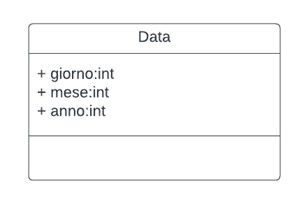
\includegraphics[width=60mm]{D3/Images/Data.jpg}
    \end{center}

\footnote{Per visualizzare le foto con una qualità maggiore si visiti il seguente link \url{https://drive.google.com/drive/folders/1yXgYDOq60fLUv0Tkpj7S3bRGar8v37Qx?usp=sharing}}

    \item \textbf{Messaggi di errore:} Viene creato anche una classe messaggi di errore, che contiene un attributo inserimento utente con tipo boolean, dato che serve un inserimento perché ci sia un messaggio di errore. Questo tipo controlla inserimento dell’utente nei campi in cui gli è richiesto di scrivere, se l’inserimento non rispetta i parametri del campo di testo, la classe annulla l'inserimento per permetterne quello corretto.
    \begin{center}
        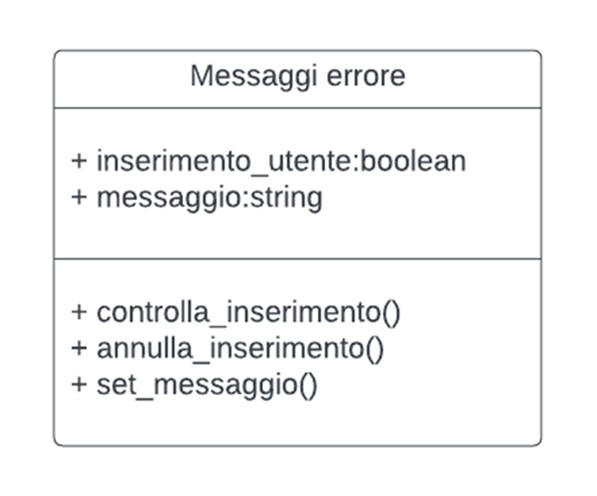
\includegraphics[width=60mm]{D3/Images/MessaggiErrore.jpg}
    \end{center}

    \item \textbf{Genere:} Viene creata una classe enum per descrivere i generi dei libri presenti in archivio, la  classe viene usata sia per la parte di ricerca/ filtri che per l’archiviazione di nuovi libri all’interno del Database
    \begin{center}
        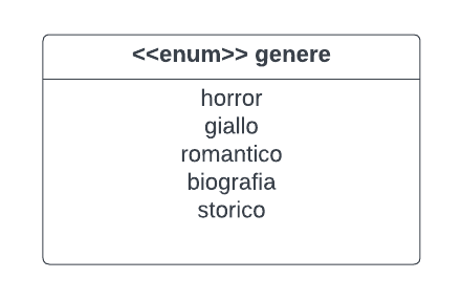
\includegraphics[width=60mm]{D3/Images/genere.png}
    \end{center}

    \item \textbf{Book:} Per gestire al meglio le funzioni della biblioteca è stato necessario creare un tipo book con le caratteristiche  dei libri presenti all’interno di EasyLib.
Gli attributi di questo tipo sono appunto: il suo titolo, genere (elencati nell’apposito enum) le informazioni dell’autore, e un Id che serve per identificare univocamente ogni singolo volume, rappresenta la chiave primaria della classe Book. Questo tipo molto importante, viene usato in quasi tutte le classi essendo un sistema bibliotecario.
    \begin{center}
        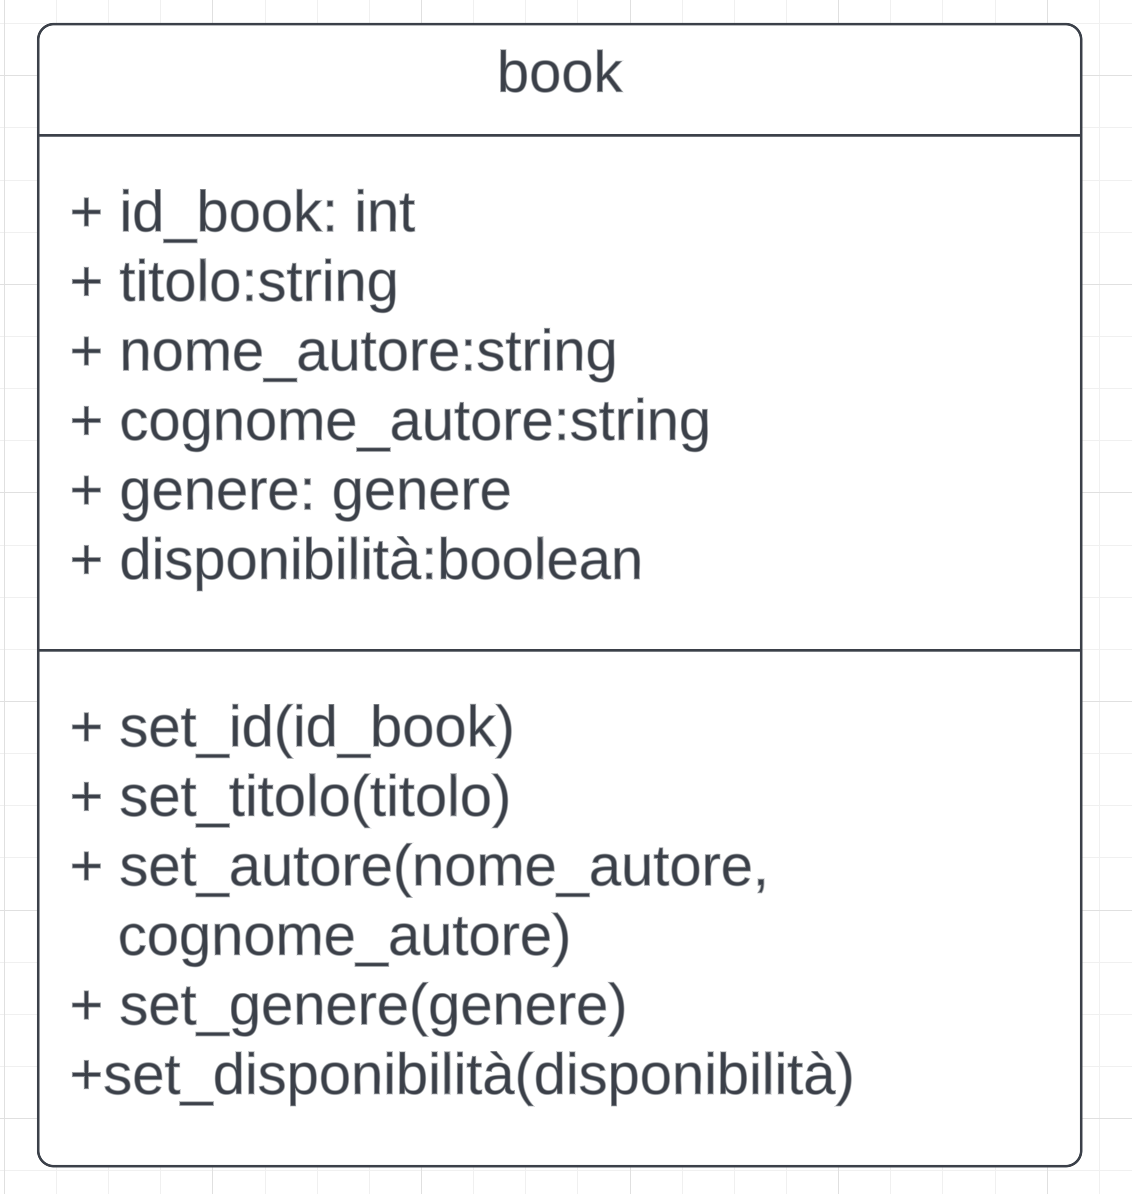
\includegraphics[width=60mm]{D3/Images/Book.png}
    \end{center}    
\end{enumerate}

\section{Classi derivate dai componenti}
In questa parte del documento vengono descritti, singolarmente o in gruppo, le varie classi ricavate dal diagramma dei componenti, dal diagramma di contesto o dai requisiti funzionali e non, dei due documenti precedenti

\subsection{Utente} 
La parte più connessa di questo diagramma delle classi, contiene tutti gli attributi che ogni utente autenticato ha all'interno dell’applicazione; le sue funzioni sono tutte quelle descritte nei documenti precedenti e verranno prese in esame una a una in seguito in questo documento. Si vuole specificare che come utente è inteso anche l’utente admin ma che in questo diagramma è stato  deciso di implementarlo come sottoclasse di un utente normale per semplificare la leggibilità del documento e farlo risultare più coeso. La classe utente ha come attributi le varie credenziali inserite alla registrazione sulla web app, e un identificativo che permette di differenziare in maniera univoca gli utenti tra loro, che è L\textbf{id\_Utente}.
\begin{center}
        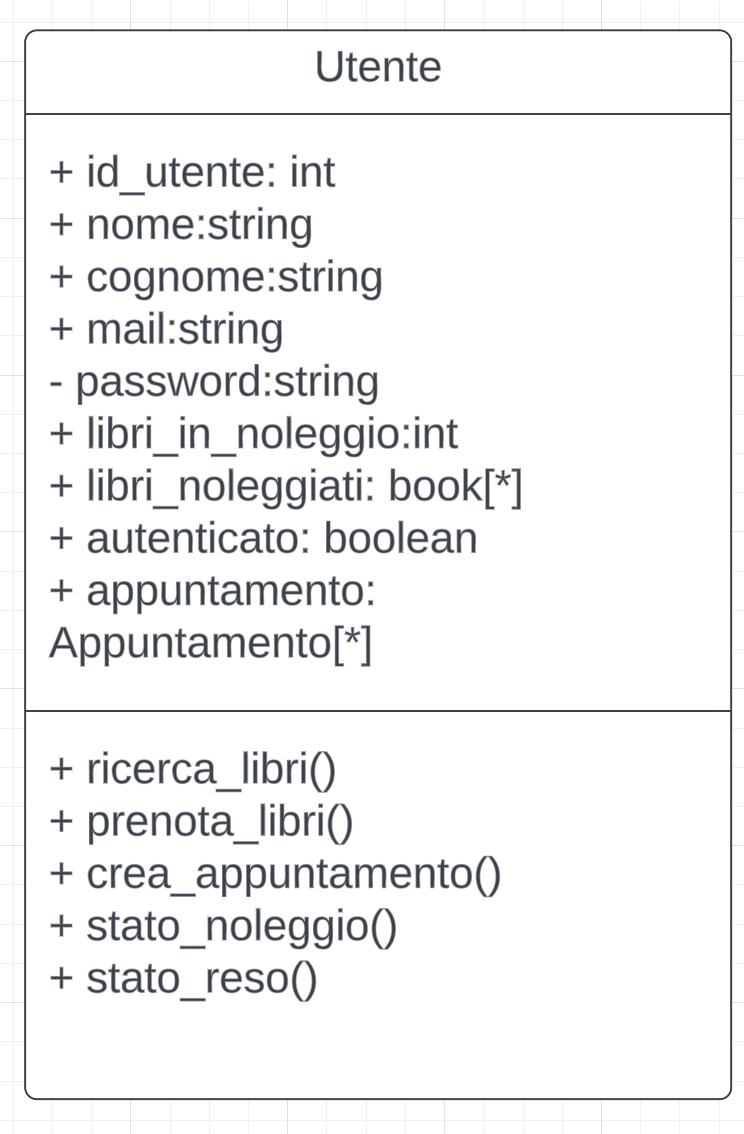
\includegraphics[width=60mm]{D3/Images/Utente.png}
\end{center}

\subsection{Database}La classe di accesso al database è stata divisa in 2 sottoclassi tramite un’aggregazione,  per riuscire a dividere meglio le funzionalità e facilitare i collegamenti, avendo i nostri due database, libri e utenti, legami con classi diverse. La superclasse DB possiede come attributo principale la sua interrogazione tramite query. Successivamente  con le funzioni di controllo nel database e invio risposta si vanno a differenziare le caratteristiche nei due rami.

\textbf{Database Utenti:}è utilizzato ogni volta che avvengono delle variazioni tra gli utenti registrati, viene usato principalmente nelle sue funzioni di modifica dall’utente amministratore.

\textbf{Database Libri:}la classe è utilizzata ogni volta che si ha bisogno di informazioni riguardanti i libri in archivio, quindi anche per una ricerca normale dell’utente, inoltre la parte di aggiunta e rimozione libri viene anche qui gestita dall’utente amministratore.
\begin{center}
        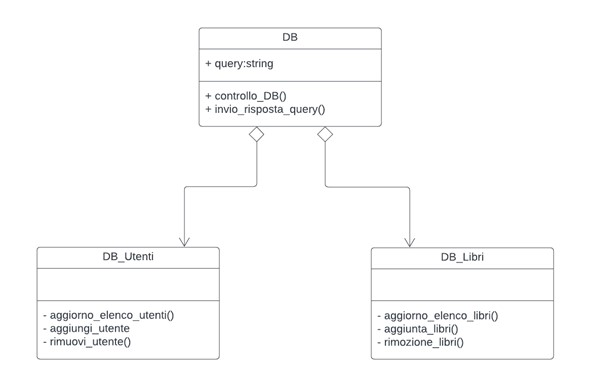
\includegraphics[width=80mm]{D3/Images/Databases.jpg}
\end{center}

\subsection{Registrazione} 
La classe registrazione gestisce la creazione di un nuovo profilo utente all’interno dell'archivio di EasyLib. gli attributi più importanti (mail, password) vengono verificati secondo i loro parametri, da le due funzioni verifica mail/password; in più la password deve rispettare i criteri di password forte ed è presente una funzione adibita a quello scopo. Si noti che la classe è direttamente collegata alla sottoclasse del database riguardante l’utente perché è li che verranno inseriti i dati registrati dai nuovi utenti.
\begin{center}
        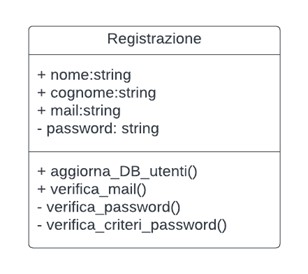
\includegraphics[width=60mm]{D3/Images/Registrazione.jpg}
\end{center}

\subsection{Autenticazione}
La classe descrive le funzioni di autenticazione, sfrutta come attributi le credenziali create in fase di registrazione, gestisce le operazioni di login e logout se l’utente non effettuerà l’operazione di logout le sue credenziali non verranno richieste finché accederà all’applicazione frequentemente. La classe ha una funzione booleana che restituisce TRUE  se le credenziali inserite dall’utente sono corrette.
\begin{center}
        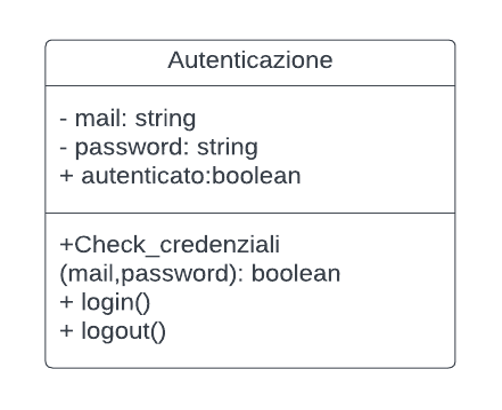
\includegraphics[width=60mm]{D3/Images/autenticazione.png}
\end{center}

\subsection{Utente-Admin} 
E’ stato deciso di rappresentare la classe admin come una sottoclasse di utente cosi da distinguere bene le funzionalità dell’admin e fare in modo che le due condividano le stesse funzioni e attributi della classe utente; va specificato che l’admin viene considerato un utente normale quando accede con le sue credenziali utente, mentre assume ruolo di amministratore e tutte le sue capacità nel momento in cui accede con le credenziali speciali admin in una schermata apposita. Il numero massimo di admin previsti per la gestione dell'applicazione è di 4 così da non avere troppe persone in grado di modificare l’applicazione. La classe admin contiene tutte le funzioni amministrative e di gestione, quali l’accesso al database libri e il controllo utenti, come rappresentato nel diagramma dei componenti.
\begin{center}
        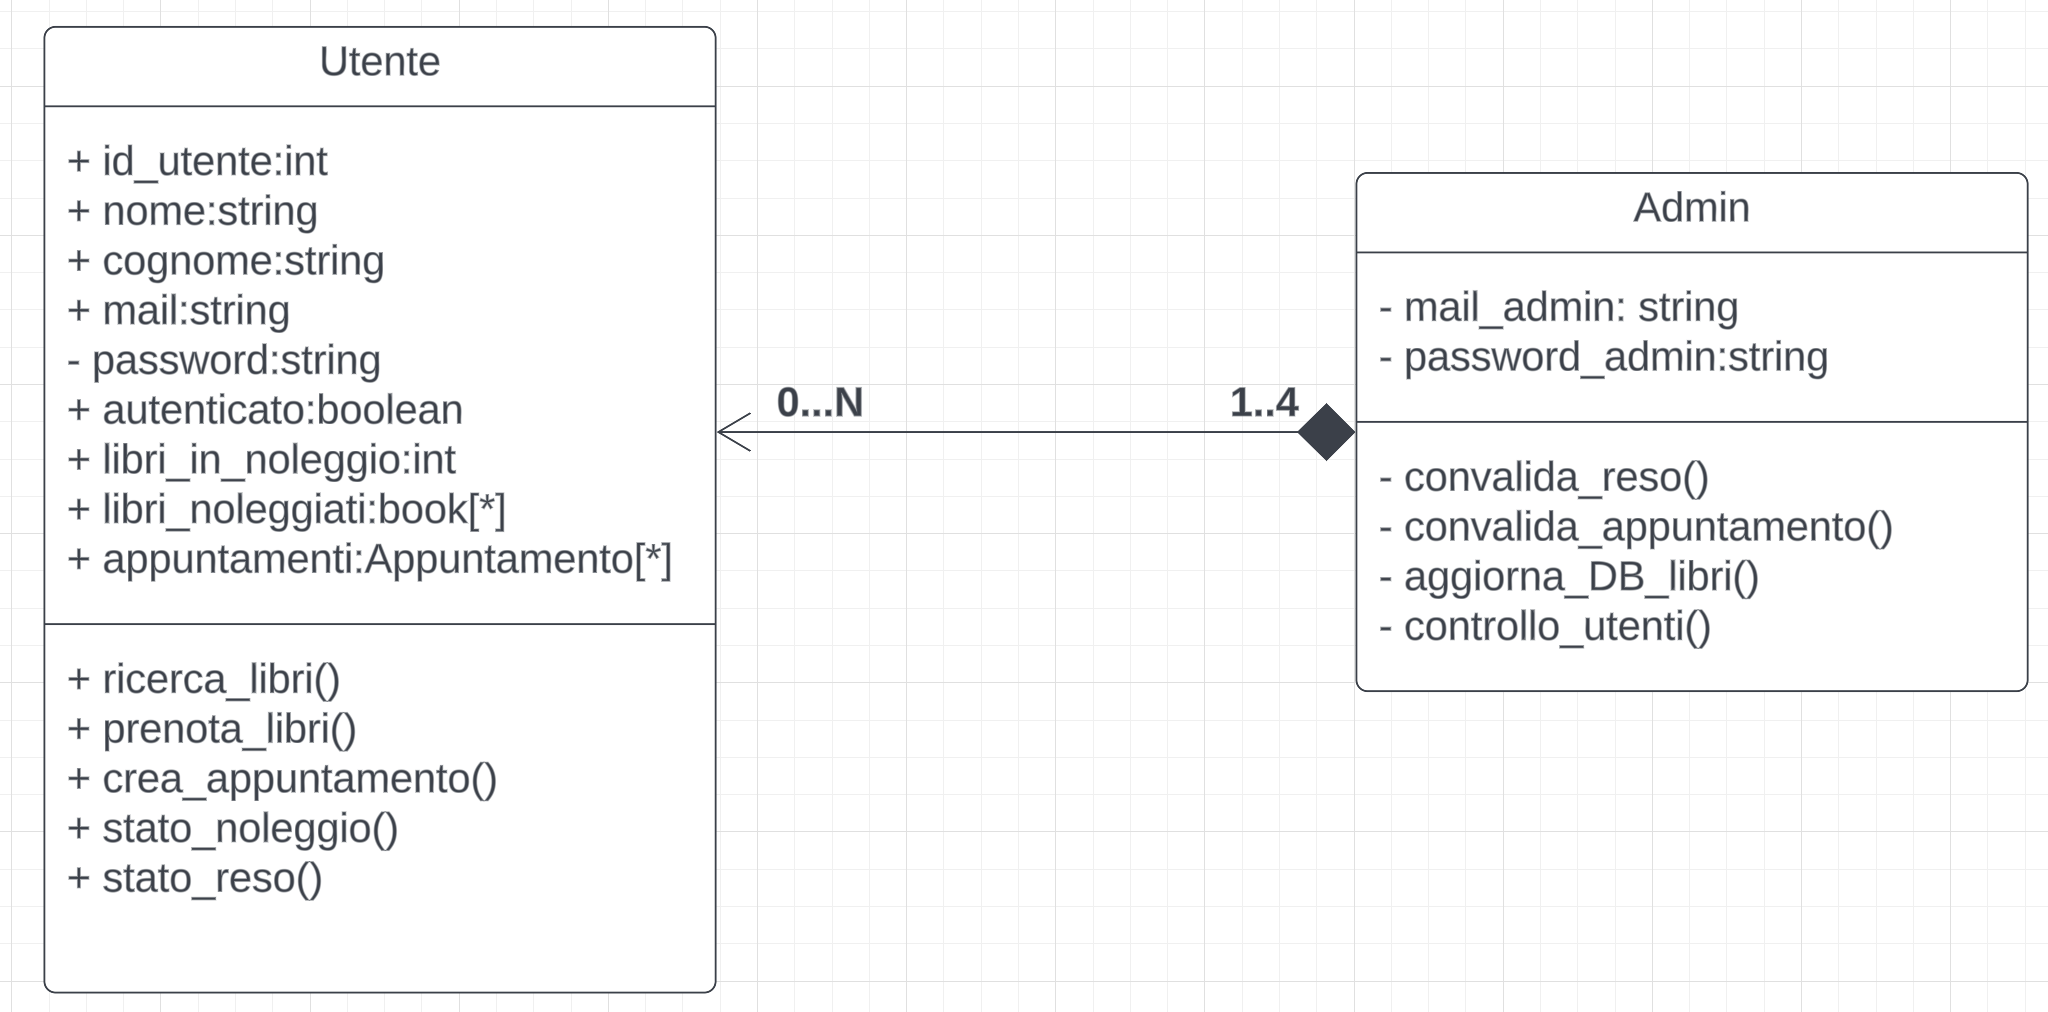
\includegraphics[width=90mm]{D3/Images/UtenteAdmin.png}
\end{center}

\subsection{Utente-ricerca,filtri}
Funzionalità più importante del nostro sistema bibliotecario è la ricerca libri, abbinata alla classe utente (ogni tipologia di utente può effettuare una ricerca libri). In questa parte viene descritta insieme alla sua classe filtri apposta creata per soddisfare le funzionalità descritte nei documenti precedenti, e che permette all’utente di cercare uno o più libri secondo al massimo tre criteri (autore, titolo, genere) descritti come attributi della  classe. Il tipo book aiuta il sistema a descrivere le informazioni riguardante i volumi e la ricerca viene affinata grazie all’enum genere, specificato all’inizio, e all’utilizzo dei 3 filtri disponibili, rappresentati come una composizione di ricerca libri, senza la ricerca infatti non avrebbe senso avere una classe filtri.
\begin{center}
        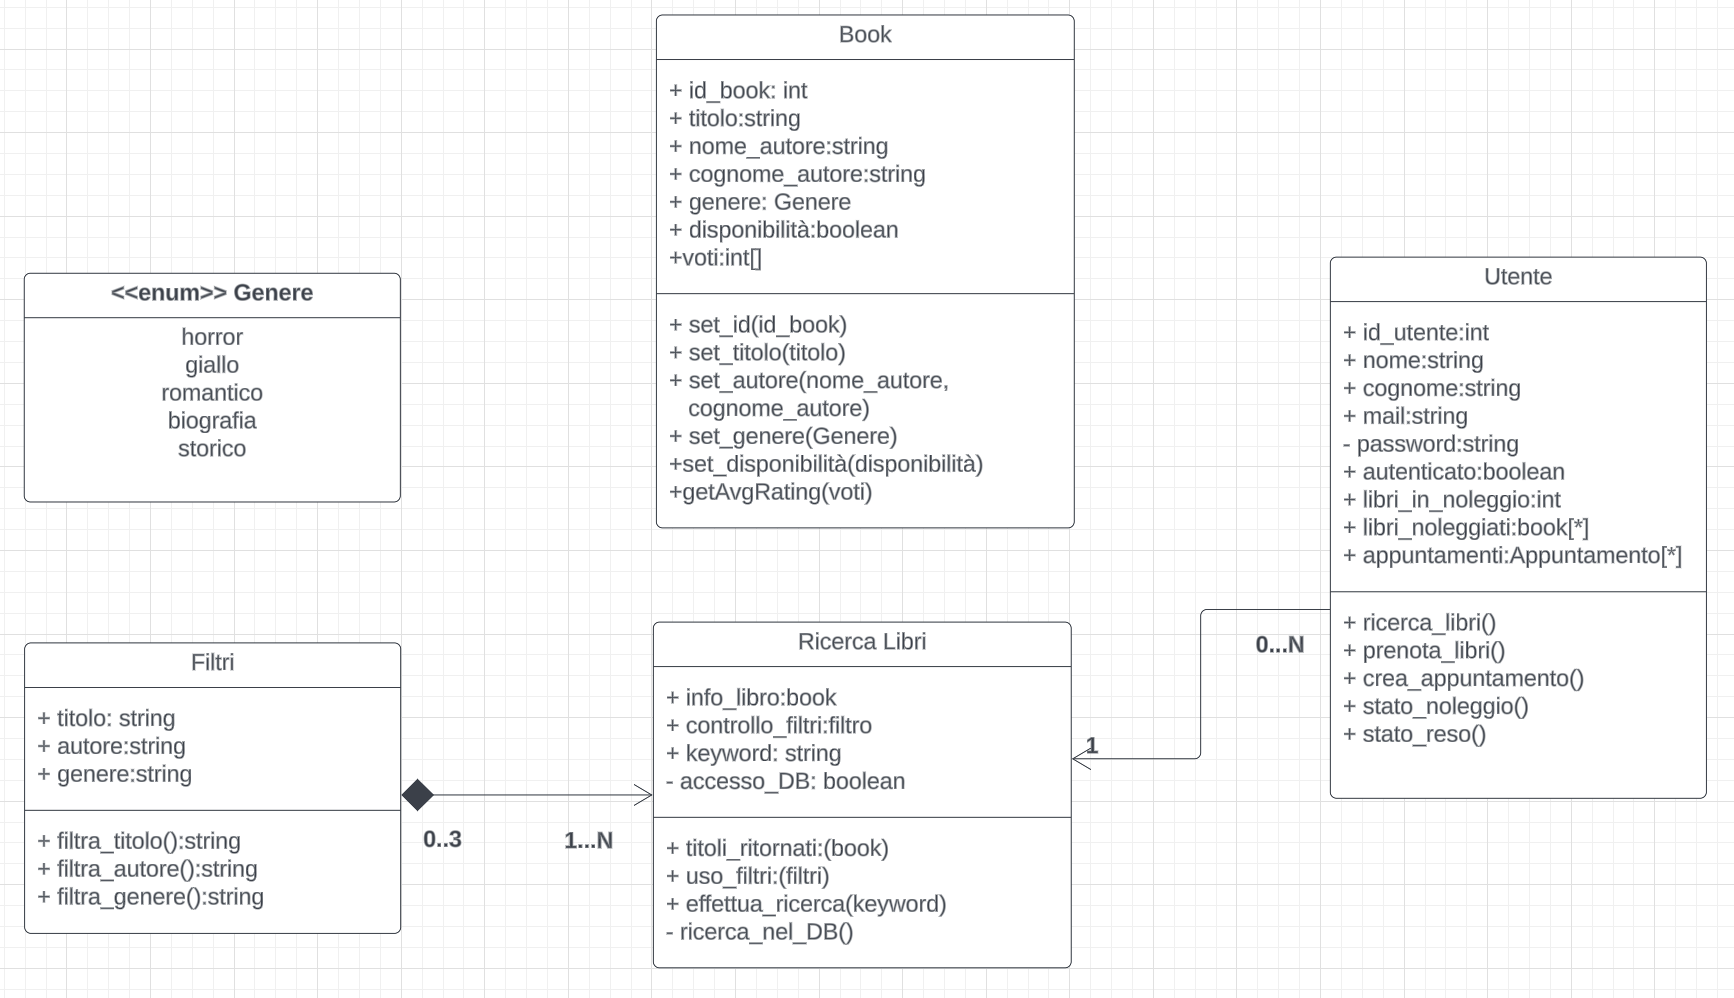
\includegraphics[width=120mm]{D3/Images/RicercaCompleta.png}
\end{center}

\subsection{Impostazioni} 
Viene introdotta una classe impostazioni che servirà all’utente autenticato per cambiare alcune specifiche della sua web app. Tra cui la lingua se italiana o inglese, descritta da un semplice attributo enumerativo, le preferenze di notifiche (se attive o meno) e la valuta in uso all’interno dell’applicazione (che verrà trattata nelle parti successive).
\begin{center}
        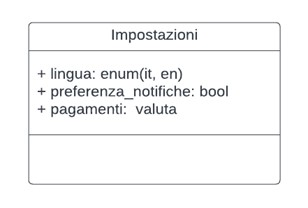
\includegraphics[width=60mm]{D3/Images/Impostazioni.jpg}
\end{center}

\subsection{Notifiche} 
La classe notifiche descrive le modalità di scambio di informazioni dall’applicazione verso l’utente. Per ogni funzionalità l’applicazione invia molteplici notifiche:  di conferma, descritte dal tipo enum notifica conferma creato appositamente, notifiche che facilitino l’interazione con l’utente, come la mail che invia il codice di quattro cifre da mostrare al momento del ritiro in fisico, oppure la mail che notifica la possibilità di valutare il libro letto, tramite una classe descritta in seguito. Ogni notifica viene inviata per mail (all'indirizzo specificato dall’utente) e possono essere disattivate le notifiche nella sezione impostazioni.  La classe nell’immagine sottostante è sgombra di collegamenti per aiutare la sua leggibilità ma va sottolineato che nel diagramma complessivo essa è fortemente connessa.
\begin{center}
        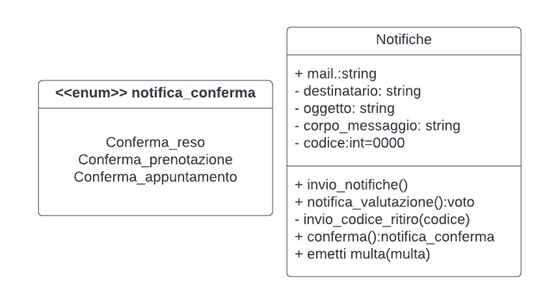
\includegraphics[width=80mm]{D3/Images/Notifiche.jpg}
\end{center}

\subsection{Donazione Libri}
Una caratteristica della nostra applicazione è la sezione di donazione libri in cui un utente può portare alla nostra sede i propri volumi vecchi. La classe in questo è descritta accoppiata alla classe admin, il cui compito è regolare le donazioni tramite gli appuntamenti di questo tipo. Dopo aver confermato l’appuntamento, che verrà descritto meglio successivamente, l’admin potrà ritirare il libro in fisico e aggiungere le sue informazioni all’interno del database, tramite le informazioni che l’utente deve fornire riguardo il libro, di tipo book, in un modulo a parte.
\begin{center}
        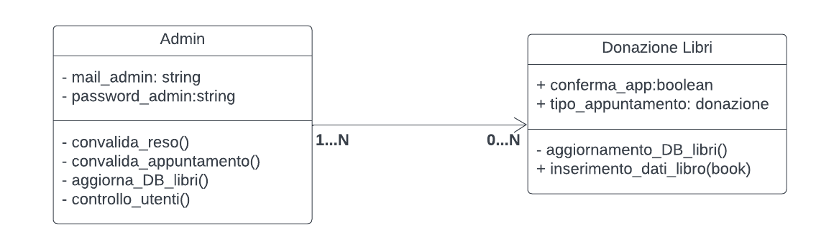
\includegraphics[width=100mm]{D3/Images/Donazione.png}
\end{center}

\subsection{Prenotazione, reso, valutazione} 
Funzionalità descritta in tutti i documenti fino ad ora è quella di prenotazione/reso. In questo caso le classi partono dall’utente che deve essere per forza autenticato, e procedono a cascata, infatti: dopo che il nostro user si è autenticato può prenotare ogni libro il cui stato è disponibile, il numero massimo di libri prenotabili è cinque. Ad avvenuta prenotazione il noleggio passerà nella classe di reso, creando la data di reso per terminare il noleggio. A reso avvenuto l’applicazione sbloccherà la funzionalità di valutazione libro (cosicché le valutazioni provengano solo da utenti che hanno noleggiato e riportato il libro) in cui l’utente potrà valutare, da una a cinque stelle, la sua lettura. Il dato verrà conservato nella sua area personale. Il codice sarà più chiaro dopo l'inserimento del codice OCL (vedi sotto).
\begin{center}
        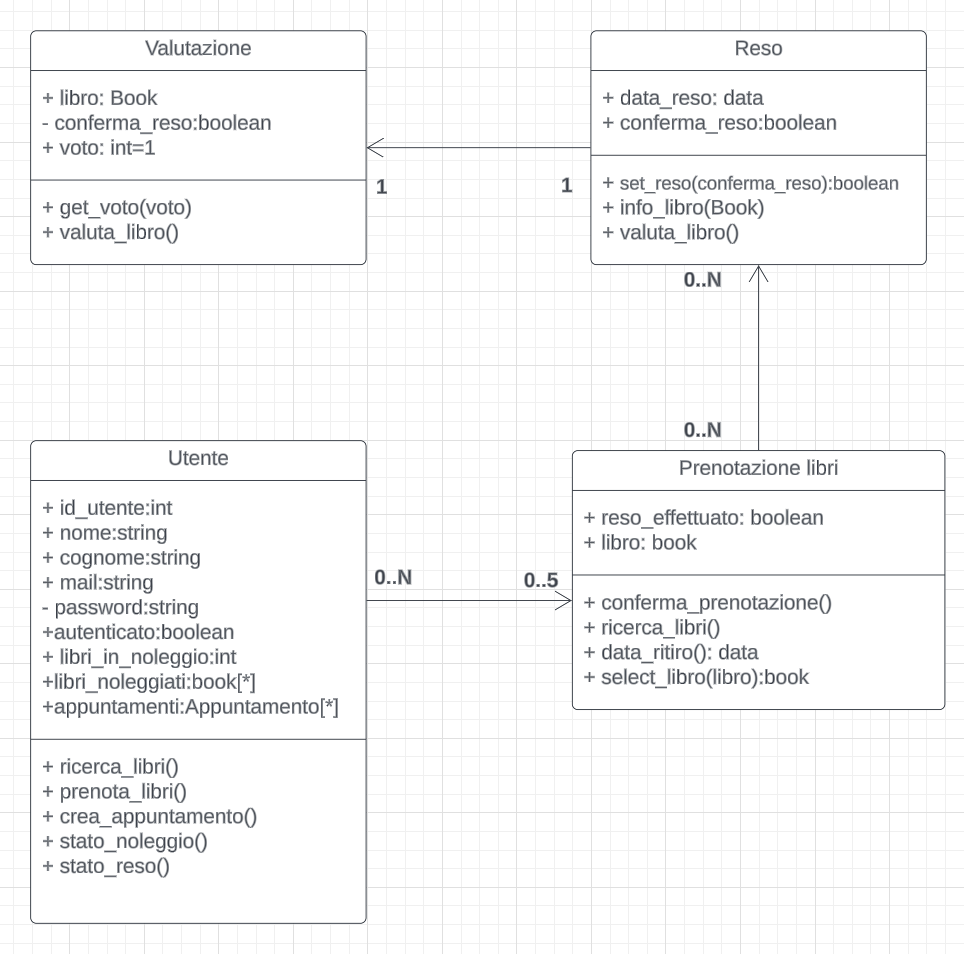
\includegraphics[width=120mm]{D3/Images/ResoPrenValutaz.png}
\end{center}

\subsection{Multa, valuta}
Nell’analisi dei componenti e del contesto viene descritta una parte di pagamento presente solo in caso di ritardo di riconsegna dei libri che invia multa come forma di tutela del sistema di biblioteca per riuscire a rientrare in possesso del volume non restituito. Queste classi descrivono le specifiche di questa funzionalità, tramite la classe \textbf{multa},  che scatta nel momento in cui scadono le 24 ore della data di reso del libro noleggiato, il sistema emette una contravvenzione inviata per mail (quella fornita dall’utente, vedi parte notifiche sopra). Un enum \textbf{valuta} permette all’utente la  scelta di con quale valuta l’utente visualizza il quantitativo della multa. 
\begin{center}
        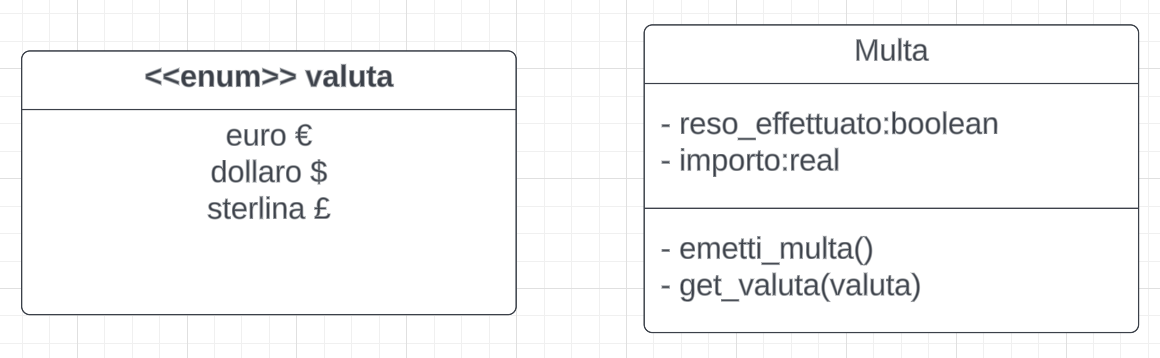
\includegraphics[width=80mm]{D3/Images/Multa.png}
\end{center}

\subsection{Appuntamento} La classe appuntamento è dotata di un attributo che ne specifica la data, e un attributo che ne specifica la tipologia; le opzioni di appuntamento sono 2 e vengono descritte nell’enum \textbf{"tipo-app"}, che è stato creato per rendere più leggibile il diagramma complessivo, esso comprende l'appuntamento per la donazione e l’appuntamento che avviene al momento del reso. Sia specificato che ogni utente può prenotare anche le 2 tipologie di appuntamento separatamente,da questo la cardinalità massima di N appuntamenti per ogni utente.
\begin{center}
        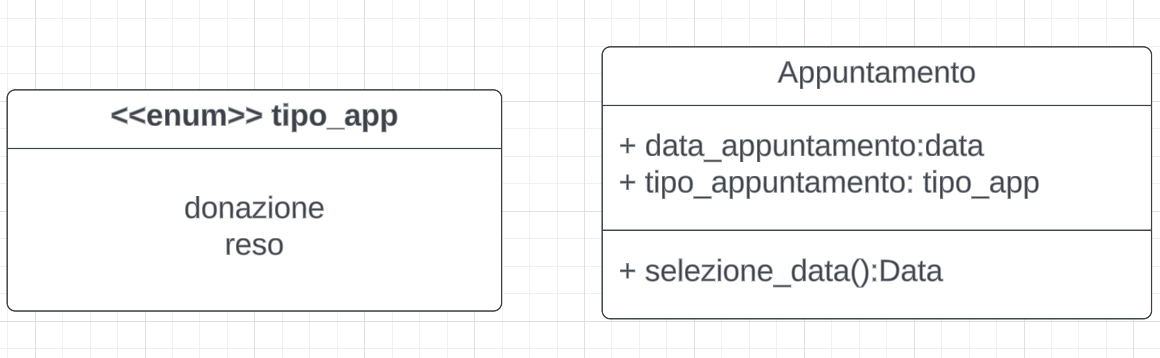
\includegraphics[width=80mm]{D3/Images/Appuntamento.png}
\end{center}

\subsection{Cancella}
la classe cancella è utile all’utente per annullare tutte le tipologie di prenotazione che può fare nel caso in cui siano state fatte per errore, o non siano più necessarie. Nel diagramma infatti è posizionata nel mezzo tra gli appuntamenti e le prenotazioni reso.
\begin{center}
        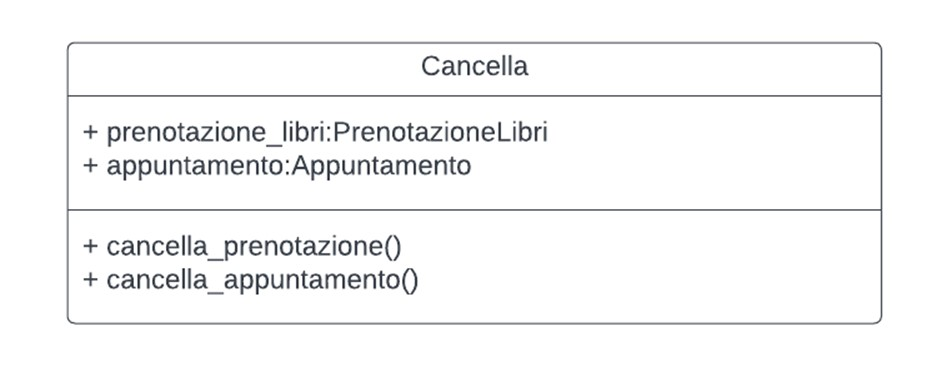
\includegraphics[width=60mm]{D3/Images/Cancella.jpg}
\end{center}

\section{Codice in Object Constraints Language (OCL)}

In questo paragrafo del documento è descritta la logica prevista su alcune operazioni di classi. Questa logica viene descritta utilizzando l’Object Constraint Language (OCL) in modo tale da esprimere queste operazioni nel contesto UML.

\subsection{Cancellazione prenotazione libri e appuntamenti}
La cancellazione degli appuntamenti e delle prenotazioni vedono coinvolte tre classi differenti.
\begin{center}
        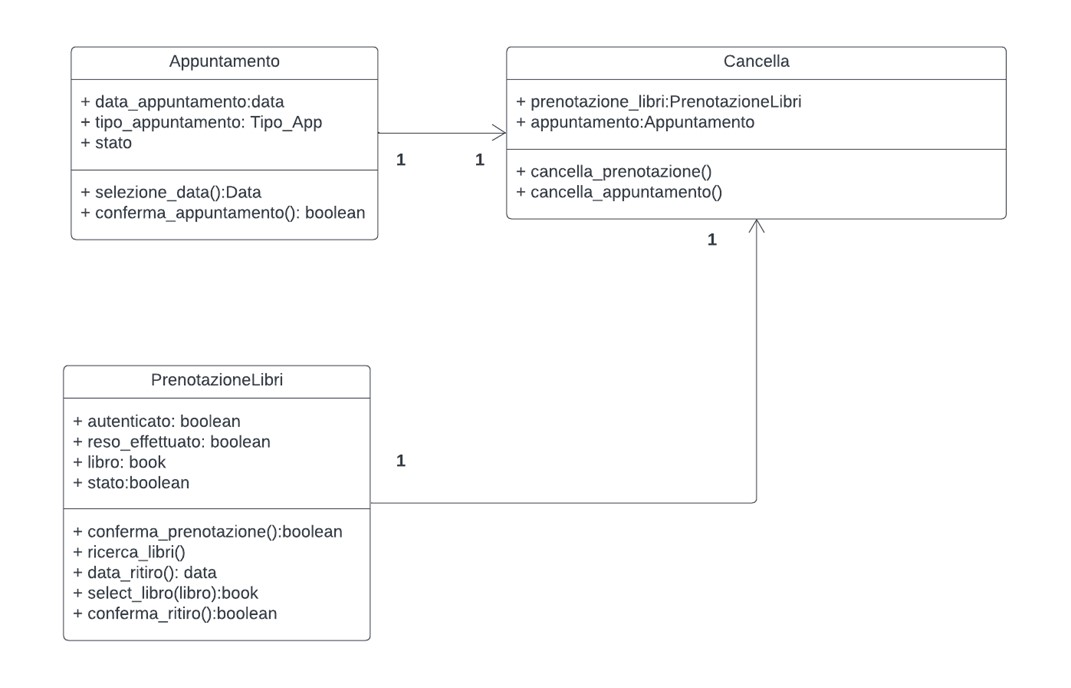
\includegraphics[width=100mm]{D3/Images/Canc_Prenot_App.jpg}
\end{center}

Le operazioni di cancella-prenotazione e cancella-appuntamento richiedono come prerequisiti che gli attributi stato della classe Appuntamento e della classe PrenotazioneLibri siano settati a TRUE, in OCL vengono espressi come di seguito
\begin{center}
        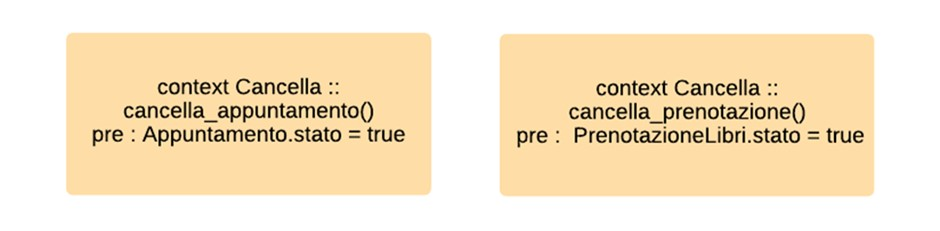
\includegraphics[width=80mm]{D3/Images/OCL_canc_pren_app.jpg}
\end{center}

\subsection{Valuta libri} 
Per effettuare il metodo valuta-libro si richiede che l’attributo conferma-reso sia uguale a TRUE. L’operazione coinvolge la classe Valutazione e viene rappresentata in OCL come segue.
\begin{center}
        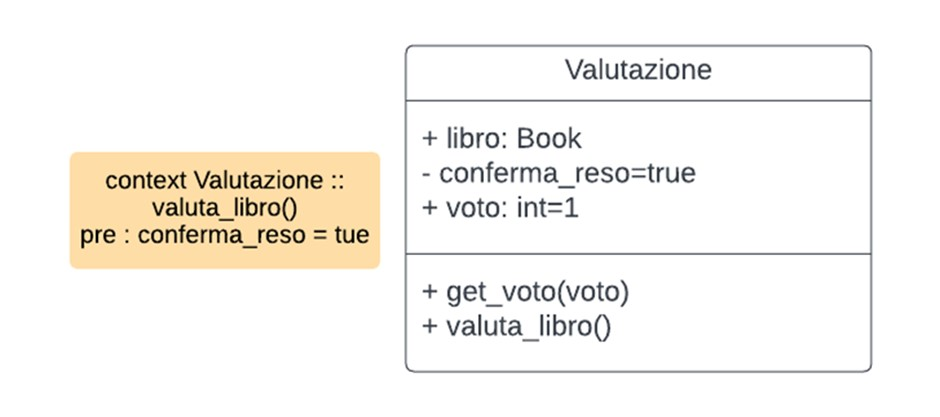
\includegraphics[width=90mm]{D3/Images/ValutazioneOCL.jpg}
\end{center}

\subsection{Emetti multa}
L’operazione emetti-multa richiede come prerequisito il fatto che l’attributo reso-effettuato sia settato false, coinvolge la classe Multa. La sua rappresentazione in OCL è la seguente:
\begin{center}
        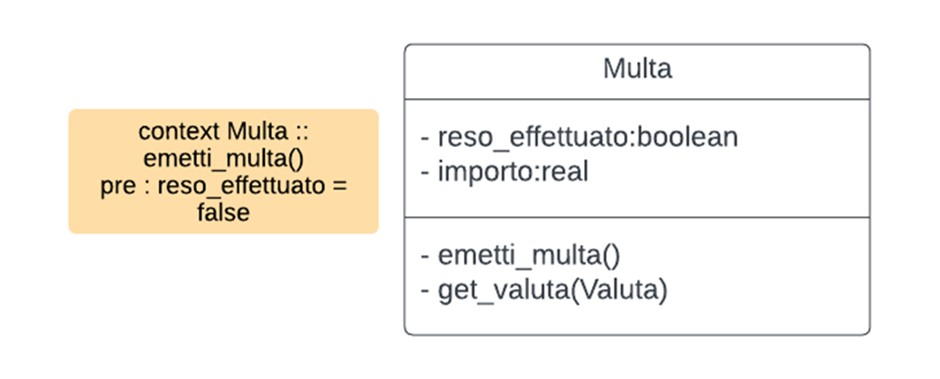
\includegraphics[width=90mm]{D3/Images/MultaOCL.jpg}
\end{center}

\subsection{Messaggi di errore e Annullamento input}
Le operazioni di annulla-inserimento e set-messaggio coinvolgono la classe Messaggi Errore vista all'inizio del documento.
Entrambe richiedono come prerequisito che l’attributo inserimento-utente venga posto a false. Vengono descritte in OCL nella seguente forma
\begin{center}
        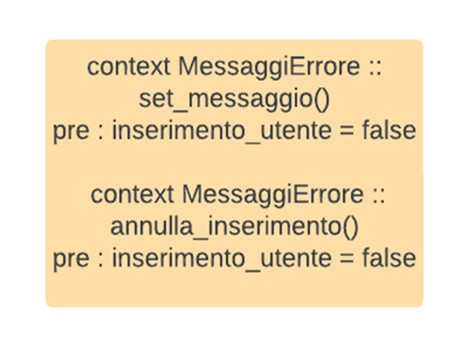
\includegraphics[width=50mm]{D3/Images/MessaggiErroreOCL.jpg}
\end{center}

\subsection{Login e Logout}
Le operazioni di login e  logout coinvolgono la classe \textbf{Autenticazione} e hanno come prerequisito che l’attributo autenticato sia settato a TRUE in OCL viene descritto come segue
\begin{center}
        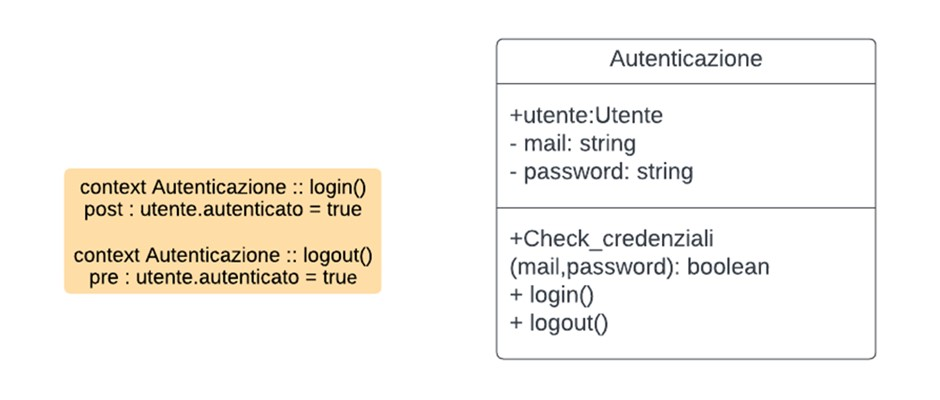
\includegraphics[width=90mm]{D3/Images/AutenticazioneOCL.jpg}
\end{center}
\subsection{Conferma reso e convalida appuntamento}
I metodi convalida-reso e convalida-appuntamento della classe \textbf{Admin} richiedono che l’attributo autenticato, derivato dalla super classe \textbf{Utente}, sia settato a TRUE ad indicare che l’utente amministratore ha fatto accesso alla sua area riservata. In OCL viene rappresentato come segue.
\begin{center}
        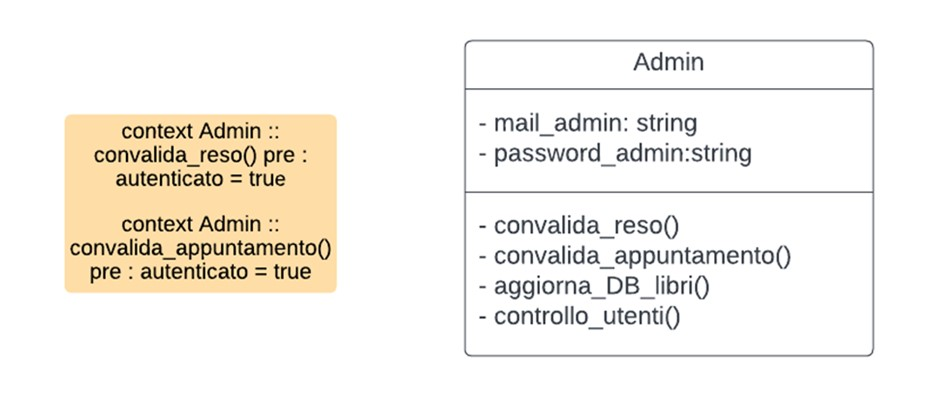
\includegraphics[width=90mm]{D3/Images/AdminOCL.jpg}
\end{center}

\subsection{Operazione della classe utente}

I metodi della classe \textbf{Utente} prenota-libri, crea-appuntamento, stato-reso, stato-noleggio e modifica-informazioni richiedono tutte come prerequisito che l’attributo autenticato sia impostato a TRUE, inoltre l’attributo libri-in-noleggio ha un vincolo per cui deve essere minore di 5, questo si riflette sul metodo prenota-libri che avrà come prerequisito anche libri\_in\_noleggio < 5. Queste operazioni sono descritte in OCL come segue
\begin{center}
        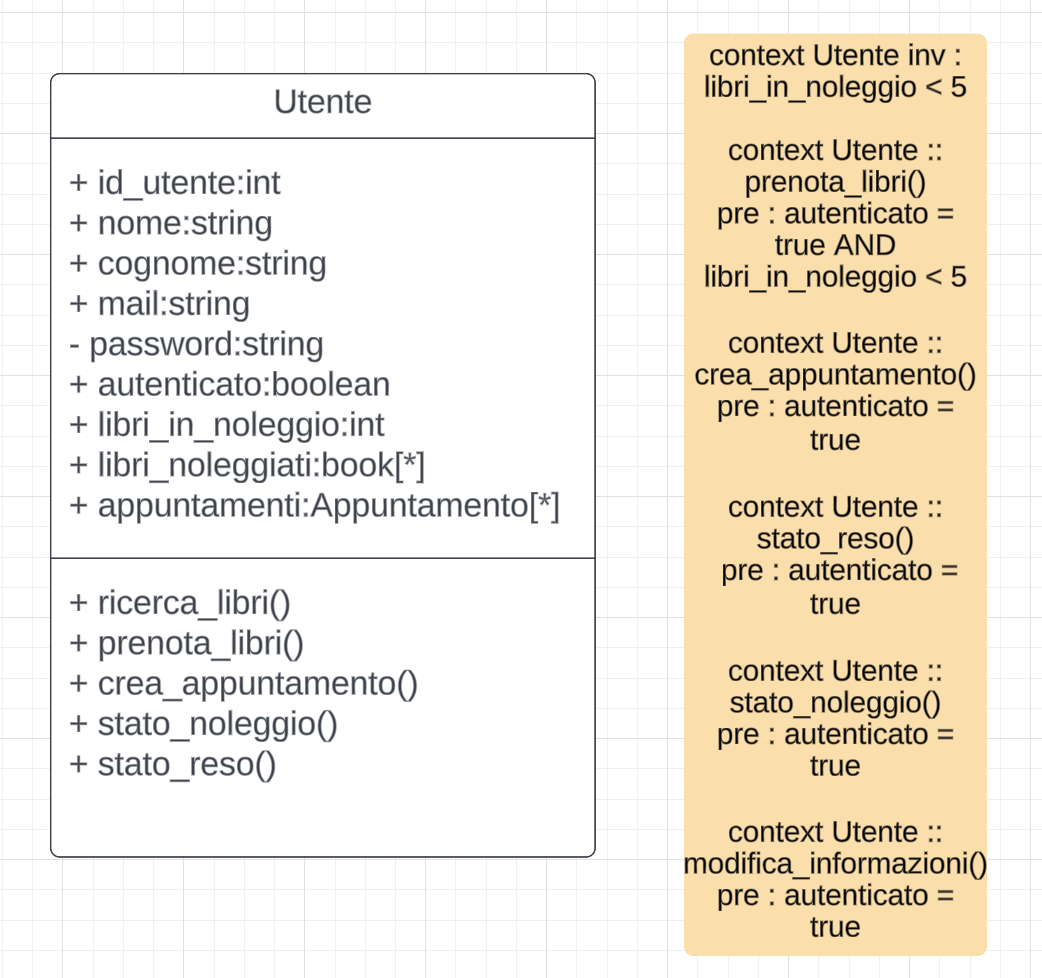
\includegraphics[width=100mm]{D3/Images/utenteOCL.png}
\end{center}

\section{Diagramma delle classi completo con codice OCL}

Infine, si riporta il diagramma delle classi completo con il codice OCL integrato.

\begin{center}
        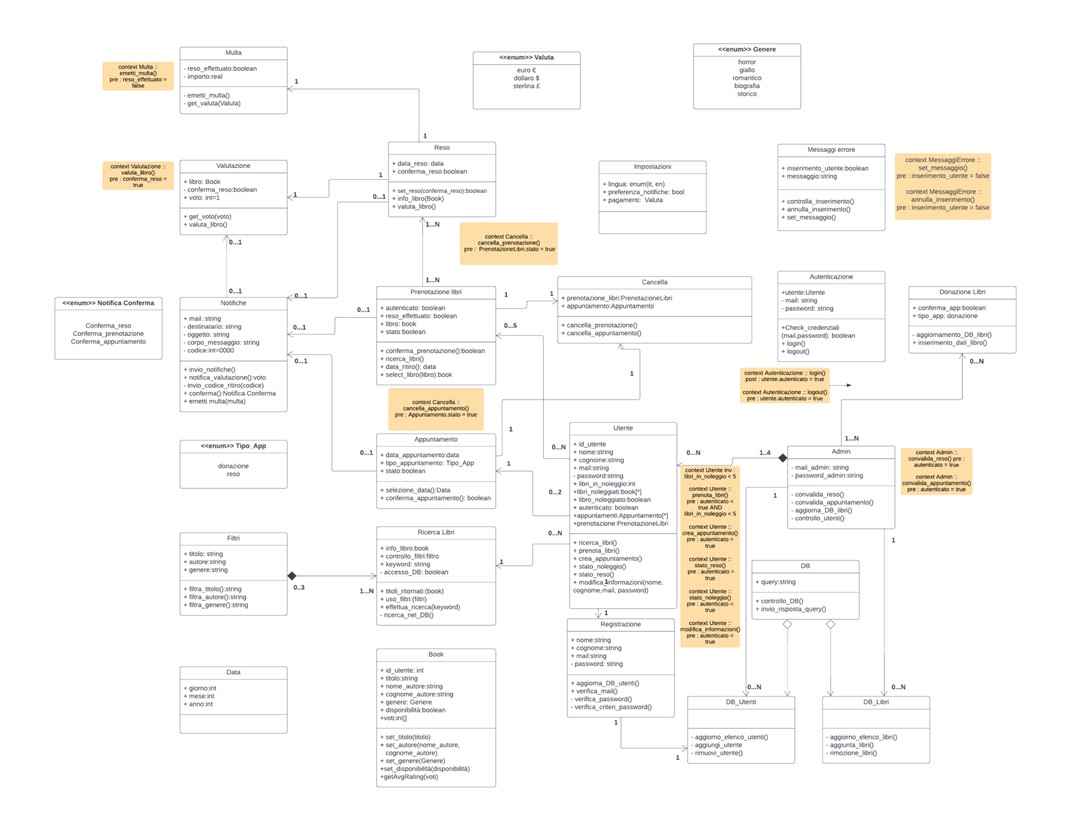
\includegraphics[width=130mm]{D3/Images/DiagrammaOCL.jpg}
\end{center}



\end{document}